% Explain the implementation of the library rust-debug

% Explain why this library was made.
Retrieving the debug information from the \gls{DWARF} sections in the \gls{elf} file is one of the main problems that needs to be solved when creating a debugger.
The \gls{DWARF} format is made to be space efficient so that the binary file doesn't get to large.
This feature of the \gls{DWARF} format has a side effect in that it makes it much more complicated for retrieving the information wanted.
Luckily there exist a library called \emph{gimli-rs}\cite{gimli} that simplifies reading the \gls{DWARF} format.
But the library still is very complicated to use because it required a lot of knowledge about the \gls{DWARF} format.
Thus the \emph{rust-debug} library was made to simplify this problem even more so that almost no knowledge of the \gls{DWARF} format is needed.


% Explain the overview of the library.
The library \emph{rust-debug} is built apone the \emph{gimli-rs} library and doesn't restrict the user from accessing the functionality of that library.
It uses the \emph{gimli-rs} library for paring the \gls{DWARF} sections into more workable data structures, the figure \ref{fig:rustdebug} shows how they are connected.
The goal of the design of the library is that a user should be able to just call a function for retrieving debug information such as a stack trace and at the same time be able to use the \emph{gimli-rs} functionality to retrieve the same information if wanted.
The library is has the features to restive the call stack, stack frames, variables, sourceinfomaiton and a function for evaluating the values of variables, the code for this library can be found in the git repository \cite{rust-debug}.


\begin{figure}[h]
	\centering
	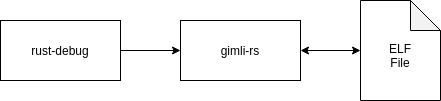
\includegraphics[width=1.0\textwidth]{rust_debug.png}
	\caption{A diagram showing the relation between the \emph{ELF} file and the two libraries \emph{rust-debug} and \emph{gimli-rs}.}
	\label{fig:rustdebug}
\end{figure}


% Explain the evaluation of source informaiton % TODO
Some of the dies have attributes that starts with \emph{DW\_AT\_decl\_}, these attributes describe which source file and where in it this dies was declared.
The library has a function for retrieving the value of all these attributes and it returns as \emph{SourceInformation} struct.
This struct contain the directory, file name, line number and column number where the die was declared in the source files.
The line and column number is very simple to retrieve because it is the same as the value of the attributes \emph{DW\_AT\_decl\_line} and \emph{DW\_AT\_decl\_column}.
It is much more complicated to get the directory and file name because the value of the attributes \emph{DW\_AT\_decl\_file} is a file index that needs to be looked up in the current units line program.
The line program indexes all the file entries and can thus be used to find the directory and file name from the file index.
If any of these attributes are not present in the die then the result of this function will be that that entry has a \emph{None} value.


% Explain the evaluation part. % TODO
% Explain the stored target memory and registers
As mention before one of the requirements for evaluating the value of a variable is access to the registers and memory of the debug target.
This library does not have that functionality because the problem of accessing memory and register is out of scope for this library.
The reason being that it would limit the number of systems it could be used for too the systems it support and also the goal of this library is to make it simpler to get debug information from \gls{DWARF}, and not to provide an interface to the systems memory and register.
That lead to the motivation of creating a data structure that holds these needed values of the system.
The implementation is just a struct with two hashmaps, one for the memory values and one for the register values.
It also has some methods for retrieving the stored values.
This struct is then used as an argument to the functions in the library and if a value that is not present in the data structure is needed the result of the function call will be a request to add the to the data structure and call the function again.
This has a negative effect in that some of the calculations will be repeated multiple times but it is not very notable.


% Explain the evaluation of vairbles.
The library has a structure called \emph{VariableCreator} which  takes a reference to the \gls{DWARF} unit and die of the variable.
Then there is a evaluation method that takes the memory and registers data structure and preforms calculation to evalue and retrieve variable information.
This method return an enum that either tell the user what memory or register values are needed, or that the it is done and the method \emph{get\_variable} can be used to get the variable.
The variable structure contains the name, value, type, sourcelocaiton and the location of where the value was evaluated from.


% Explain the evaluation of call stack % TODO
% Explain the evaluation of stackframe 
Using the call stack result each call frame can be used to create a stack frame.
These stack frames are like the call frames except that they have more information like the function name of the frame, where the function was declared and the value of all the variables.
The way this library  constructs a \emph{StackFrame} struct works the same way as when creating a variable.
Meaning that there is a helper struct for creating the stack frame which requires the memory and register struct as an argument.
This helper struct when created will find the name of the function for this frame and where it was declared, then it will go through all dies that belong to that function to find all the variable dies and store it in a list.
This list of variable dies is then used to evaluate all variables and each entry is removed when evaluated and the result stored in a variables attribute.
Thus if one of the variables requires a value from memory that is not present in the memory and register struct then all the variables already evaluated doesn't need to be evaluated again.
The evaluating of the variables is done in the same way as describe above the only difference is that the registers values is set to be the ones evaluated in the call frame.
Thus adding the value of a register to the memory and register struct won't do anything when evaluating a stack frame.
Then lastly the stack frame can be retrieve using the method \emph{get\_stack\_frame} from the stack frame helper struct.


% Explain how to get breakpoint locaiton.
There is also a function for finding out what machine code address a certain line in a source file corresponds to.
It works by first finding out which compilation unit that the source file corresponds to by looping trough all the file entries in all of the compilation units. 
Then it loops through all the rows in that file entry and adds all the rows that match the source line number.
If the vector is empty after that then there is no machine code instruction that matches that source line otherwise it is not empty there is at least one instruction that corresponds to that line.
When there are multiple match the function will take the one that has the nearest column value to the source lines column value.

